\documentclass[titlepage, fleqn, a4paper, 12pt, twoside]{article}
\usepackage{exsheets} %question and solution environments
\usepackage{amsmath, amssymb, amsthm} %standard AMS packages
\usepackage{esint} %integral signs
\usepackage{marginnote} %marginnotes
\usepackage{gensymb} %miscellaneous symbols
\usepackage{commath} %differential symbols
\usepackage{xcolor} %colours
\usepackage{cancel} %cancelling terms
\usepackage[free-standing-units]{siunitx} %formatting units
\usepackage{tikz, pgfplots} %diagrams
	\usetikzlibrary{calc, hobby, patterns, intersections, angles, quotes, spy}
\usepackage{graphicx} %inserting graphics
\usepackage{epstopdf} %converting and inserting eps graphics
\usepackage{hyperref} %hyperlinks
\usepackage{datetime} %date and time
\usepackage{ulem} %underline for \emph{}
\usepackage{xfrac, lmodern} %inline fractions
\usepackage{enumerate, enumitem} %numbered lists
\usepackage{float} %inserting floats
\usepackage[american voltages]{circuitikz} %circuit diagrams
\usepackage{pdflscape} %pages in landscape orientation
\usepackage{setspace} %double spacing
\usepackage{microtype} %micro-typography
\usepackage{listings} %formatting code
	\lstset{language=Matlab}
	\lstdefinestyle{standardMatlab}
	{
		belowcaptionskip=1\baselineskip,
		breaklines=true,
		frame=L,
		xleftmargin=\parindent,
		language=C,
		showstringspaces=false,
		basicstyle=\footnotesize\ttfamily,
		keywordstyle=\bfseries\color{green!40!black},
		commentstyle=\itshape\color{purple!40!black},
		identifierstyle=\color{blue},
		stringstyle=\color{orange},
	}
\usepackage{algpseudocode} %algorithms
\usepackage{algorithm} %algorithms
\usepackage{chronology}
\usepackage{qtree}
\usepackage{varwidth}
\usepackage{asymptote}
\usepackage{setspace}
\usepackage{titlesec}
\usepackage{ifdraft}
\usepackage{booktabs}
	\ifoptiondraft
	{%
		\doublespacing
		\usepackage{showframe}
	}
	{%
	    % nothing to be done here
	}
\usepackage{todonotes}
%\usepackage{syntonly}
%\syntaxonly

\newcommand\numberthis{\addtocounter{equation}{1}\tag{\theequation}} %adds numbers to specific equations in non-numbered list of equations

\theoremstyle{definition}
\newtheorem{example}{Example}
\newtheorem{definition}{Definition}

\theoremstyle{theorem}
\newtheorem{theorem}{Theorem}
\newtheorem{law}{Law}

%\renewcommand{\Re}{\mathrm{Re}}
%\renewcommand{\Im}{\mathrm{Im}}

\DeclareMathOperator{\Arg}{Arg}

\DeclareMathOperator{\Int}{Int}
\DeclareMathOperator{\Ext}{Ext}
\DeclareMathOperator{\boundary}{\partial}

\DeclareMathOperator{\Log}{Log}
\DeclareMathOperator{\pv}{pv}

\DeclareMathOperator{\length}{length}

\DeclareMathOperator{\Res}{Res}

\makeatletter
\@addtoreset{section}{part} %resets section numbers in new part
\makeatother

\newcommand\blfootnote[1]{%
	\begingroup
	\renewcommand\thefootnote{}\footnote{#1}%
	\addtocounter{footnote}{-1}%
	\endgroup
}

\renewcommand{\marginfont}{\scriptsize \color{blue}}

\renewcommand{\tilde}{\widetilde}

\SetupExSheets{solution/print = true} %prints all solutions by default

%opening
\title{Complex Functions : Review Session}
\author{Aakash Jog}
\date{2015-16}

\begin{document}

\maketitle
%\setlength{\mathindent}{0pt}

\blfootnote
{	
	\begin{figure}[H]
		
\includegraphics[height = 12pt]{cc.eps}
		
\includegraphics[height = 12pt]{by.eps}
		\includegraphics[height = 12pt]{nc.eps}
		
\includegraphics[height = 12pt]{sa.eps}
	\end{figure}
	This work is licensed under the Creative Commons Attribution-NonCommercial-ShareAlike 4.0 International License. To view a copy of this license, visit \url{http://creativecommons.org/licenses/by-nc-sa/4.0/}.
} %CC-BY-NC-SA license

\begin{question}{10}
	Let
	\begin{align*}
		D & = \left\{ z \in \mathbb{C} : \Re(z) \ge 0 \right\}
	\end{align*}
	Is $f(z) = \cos z$ bounded, where $f : D \to \mathbb{C}$?
\end{question}

\begin{solution}
	\begin{align*}
		\cos z & = \frac{e^{i z} - e^{-i z}}{2} \\
                       & = \frac{e^{i x} e^{-y} - e^{-i x} e^y}{2}
	\end{align*}
	Therefore, if $x = 0$,
	\begin{align*}
		\cos z                                           & = \frac{e^{-y} + e^y}{2} \\
		\therefore \lim\limits_{y \to \pm \infty} \cos z & = \infty
	\end{align*}
	Therefore, $\cos z$ is not bounded.
\end{solution}

\begin{question}{15}
	$f$, $g$, $h$ are entire, such that $\forall n \in \mathbb{N}$,
	\begin{align*}
		f\left( 1 + \frac{\pi}{n} \right) & = \cos\left( 1 + \frac{\pi}{n} \right) \\
		g(2 \pi n)                        & = \cos(2 \pi n)                        \\
		h\left( \frac{\pi i}{n} \right)   & = \cosh\left( \frac{\pi}{n} \right)
	\end{align*}
	Two of these functions are necessarily identical to each other, and the third is not necessarily identical to the other two.
	Determine which two are identical, and explain.
	Explain why the third is not necessarily identical to the other two.
\end{question}

\begin{solution}
	Let
	\begin{align*}
		z_n & = 1 + \frac{\pi}{n}
	\end{align*}
	Therefore, as $\{z_n\}$ converges to $1$, and as
	\begin{align*}
		f(z_n) & = \cos(z_n)
	\end{align*}
	by the Second Identity Theorem,
	\begin{align*}
		f(z) & \equiv \cos(z)
	\end{align*}
	~\\
	Let
	\begin{align*}
		z_n & = \frac{\pi i}{n}
	\end{align*}
	Therefore,
	\begin{align*}
		\cos\left( \frac{\pi i}{n} \right) & = \frac{e^{-\frac{\pi}{n}} + e^{\frac{\pi}{n}}}{2} \\
                                                   & = \cosh\left( \frac{\pi}{n} \right)
	\end{align*}
	Therefore, as $\{z_n\}$ converges to $0$, and as
	\begin{align*}
		h(z_n) & = \cos(z_n)
	\end{align*}
	by the Second Identity Theorem,
	\begin{align*}
		h(z)                                       & \equiv \cos(z)                            \\
		\therefore h\left( \frac{\pi i}{n} \right) & \equiv \cos\left( \frac{\pi i}{n} \right) \\
                                                           & \equiv \cosh\left( \frac{\pi}{n} \right)
	\end{align*}
	~\\
	Therefore,
	\begin{align*}
		f & \equiv h
	\end{align*}
	$g$ is not necessarily identical to the other two, as the same argument cannot be used for $g$, as the sequence $\{2 \pi n\}$ does not converge.
\end{solution}

\begin{question}{13}
	Develop the Laurent series of
	\begin{align*}
		g(z) & = \frac{1}{z^2 (z - i) (z - 1 - i)}
	\end{align*}
	around $z = 0$ in the ring $1 < |z| < 2$.
\end{question}

\begin{solution}
	\begin{align*}
		\frac{1}{(z - i) (z - 1 - i)} & = \frac{-1}{z - i} + \frac{1}{z - 1 - i}
	\end{align*}
	Therefore,
	\begin{align*}
		g(z) & = \frac{1}{z^2} \frac{1}{z - i} + \frac{1}{z^2} \frac{1}{z - 1 - i}
	\end{align*}
	Let
	\begin{align*}
		g_1(z) & = \frac{1}{z^2} \frac{1}{z - i} \\
		g_2(z) & = \frac{1}{z^2} \frac{1}{z - 1 - i}
	\end{align*}
	Therefore,
	\begin{align*}
		g_1(z)  & = -\frac{1}{z^3} \frac{1}{1 - \frac{i}{z}}                    \\
		\marginnote
		{
			As $\left| \frac{i}{z} \right| < 1$, the infinite summation of $\frac{i^n}{z^n}$ is $\frac{1}{1 - \frac{i}{z}}$.
		}      \\
                        & = -\frac{1}{z^3} \sum\limits_{n = 0}^{\infty} \frac{i^n}{z^n} \\
                        & = \sum\limits_{n = 0}^{\infty} -\frac{i^n}{z^{n + 3}}         \\
                        & = \sum\limits_{n = 3}^{\infty} -\frac{i^{n - 3}}{z^n}
	\end{align*}
	Therefore,
	\begin{align*}
		g_2(z) & = \frac{1}{z^2} \frac{1}{z - (1 + i)}                                       \\
                       & = -\frac{1}{(1 + i) z^2} \frac{1}{1 - \frac{z}{1 + i}}                      \\
                       & = -\frac{1}{(1 + i) z^2} \sum\limits_{n = 0}^{\infty} \frac{z^n}{(1 + i)^n} \\
                       & = \sum\limits_{n = 0}^{\infty} \frac{-z^{n - 2}}{(1 + i)^{n + 1}}           \\
                       & = \sum\limits_{n = -2}^{\infty} \frac{-z^n}{(1 + i)^{n + 3}}
	\end{align*}
\end{solution}

\begin{question}{10}
	$f$ is analytic in $\overline{D_{0,3}}$, satisfying
	\begin{align*}
		\left| f(z) \right| & \le \left| \frac{1}{z^2} \right|
	\end{align*}
	for all $z \in \overline{D_{0,3}}$.
	Prove that $\forall z \in \overline{D_{0,3}}$,
	\begin{align*}
		\left| f(z) \right| & \le \frac{1}{9}
	\end{align*}
\end{question}

\begin{solution}
	As $\frac{1}{z^2}$ is not analytic, the maximum modulus principle cannot be applied, and hence it cannot be bounded.\\
	Let
	\begin{align*}
		g(z) & = f(z) z^2
	\end{align*}
	Therefore, as both $f(z)$ and $z^2$ are analytic, $g(z)$ is also analytic.
	Therefore, $\forall z \in \overline{D_{0,3}}$,
	\begin{align*}
		\left| g(z) \right| & = \left| f(z) \right| \left| z^2 \right| \\
                                    & \le 1
	\end{align*}
	Therefore,
	\begin{align*}
		\max\limits_{z \in \overline{D_{0,3}}} \left| g(z) \right| & = \max\limits_{z \in \partial D_{0,3}} \left| g(z) \right|                    \\
                                                                           & = \max\limits_{z \in \partial D_{0,3}} \left| f(z) \right| \left| z^2 \right| \\
                                                                           & = 9 \max\limits_{z \in \partial D_{0,3}} \left| f(z) \right|
	\end{align*}
	Therefore,
	\begin{align*}
		\max\limits_{z \in \overline{D_{0,3}}} \left| f(z) \right| & = \max\limits_{z \in \partial D_{0,3}} \left| f(z) \right| \\
                                                                           & \le \frac{1}{9}
	\end{align*}
\end{solution}

\begin{question}{14}
	\begin{align*}
		f(z) & = \frac{\sin(i \pi z)}{(z - 1) \left( z^4 - 1 \right)}
	\end{align*}
	Find the isolated singular points of $f$ and determine their types.
\end{question}

\begin{solution}
	The points $z = \pm 1$ and $z = \pm i$ are isolated singular points of $f$.\\
	Therefore, $\lim\limits_{z \to 1} f(z) (z - 1)^2$ is finite and non-zero.
	Therefore, $z = 1$ is a pole of order $2$.\\
	Therefore, $\lim\limits_{z \to -1} f(z) (z + 1)$ is finite and non-zero.
	Therefore, $z = -1$ is a pole of order $1$.\\
	Similarly, as the limits of the function at $\pm i$ are finite, $\pm i$ are removable isolated singular points.
\end{solution}

\begin{question}{11}
	\begin{align*}
		f(z) & = \frac{\sin(i \pi z)}{(z - 1) \left( z^4 - 1 \right)}
	\end{align*}
	Calculate $\displaystyle \int\limits_{C_{1,\sqrt{3}}} f(z) \dif z$.
\end{question}

\begin{solution}
	The isolated singular points of $f(z)$ are $\pm 1$ and $\pm i$.
	Therefore, as $\pm i$ and $1$ are in $D_{1,\sqrt{3}}$,
	\begin{align*}
		\int\limits_{C_{1,\sqrt{3}}} f(z) \dif z & = 2 \pi i \left( \Res_{f}(1) + \Res_{f}(i) + \Res_{f}(-i) \right)
	\end{align*}
\end{solution}

\end{document}
